\section{Workloads, numerical coverage and statistical reconstruction}
\label{sec:supp-design}
The CUDA references bind a whole-prompt caller with physical microbatch one and last-only prompt output; the controlled SmolLM2 Vulkan appends retain outer prompt calls of up to 512 tokens and physical microbatch 128. The main configurations use one dense nonwrapping sequence, F16 K/V, greedy generation and non-Flash causal attention. Known-query work uses up to 32 positions. A different model, device, producer or numerical module defines a different reference.

The historical Linux Qwen/Smol reports describe comparisons of complete requested vectors and active K/V by layer and logical position. Their geometry cases cover widths 1, 4, 8 and 32, inside and crossing prefixes, tails and the tested output masks. Natural cases exercise early and later rejection, trim, pending correction and bonus tokens, native end-of-generation, caps and reset. The Llama deployment has a separately established reference. These historical observations are retained as reported qualification, rather than an independent replay of the original native records. The 32B strong-control record directly identifies full 151,936-entry output and 64-layer active-state comparisons at its tested boundaries.

The wide-verification study initially freezes source, order and analysis before 1,024 clean timings and 128 primers. A mask-reader correction is validated offline and the completed first worker is retained without rerunning the GPU; its gap remains in the worker accounting. A later joint boundary/rollback qualification on an exposed natural root adds 1,936 full-vector and 296 active-target-KV comparisons across all eight arms. These later observations extend the checked transitions, not the diagnostic coverage of the earlier clean runs.

APPS and MATH provide the natural Qwen task identities~\cite{apps,math}. Qwen 8B and 14B share 16 roots and four sessions. Llama uses 12 roots selected after excluding previous project exposure. Each six-arm panel has two separate primer requests per worker; its 48 primers are not inference units. Four-arm factorials use four Williams rows, with 256 formal requests and 32 primers per model. The original 8B two-D4 order is fixed; its compound contrast therefore retains an order confound that the later balanced factorial does not. Model hashes, prompt IDs and orders are linked in the source index.

The 32B strong comparison uses 12 roots, six coding and six mathematics, four rounds and three arms. Its 144 measured requests each follow a matched warmup. Root-level paired log ratios are averaged equally; the bootstrap resamples the two six-root strata separately. Its primary C/B interval uses 95\% coverage and secondary G comparisons 97.5\%. Q8 application and factorial intervals use 99\% coverage for their five-comparison families. Repeated sessions travel with the root under resampling. These intervals condition on the observed sessions.

The natural multi-turn pilot uses two OpenAssistant development conversations~\cite{oasst}, two rounds and eight measured episodes. Its canonical transition does not initially retain the currently generated body as reusable KV; an earlier canonical prefix can be reused on later turns. This protocol creates less local-cut opportunity than assuming that every generated body persists. Its pooled ratio is descriptive. The dataset revision's card and license identify Apache-2.0. The package includes public timing records and diagnostic projections, including short token and text excerpts used to explain the history transition; it does not bundle the full conversation corpus.

\paragraph{Reconstruction levels.}
The supplied 8B/14B/Llama service and factorial files contain 1,568 measured timing rows. The 32B strong file includes 144 warm and 144 measured rows; the multi-turn file has eight measured episodes. The CPU routines preserve original root order, bootstrap seeds and estimands. Separate NumPy and standard-library implementations agree to $2\times10^{-12}$ in the reconstructed statistics. This tolerance concerns arithmetic in the statistical analysis, not numerical compatibility of inference. Other legacy panels supply the public numeric projections or root aggregates identified in their manifests; availability of those projections does not imply availability of all native receipts.

\section{Strong-control phase account and sensitivity}
\label{sec:supp-s3}
The S3 phase account sums the same 48 measured requests in each arm. The timers partition the resident-service clock: prefill and decode include their nested backend quantization, kernels and synchronization. Those nested activities were not separately timed. Table~\ref{tab:supp-s3-phase} shows why the service reduction is concentrated in prefill. It is descriptive accounting of the original panel, not a new set of independent phase samples.

\begin{table}[htbp]
\centering\small
\caption{S3 host-phase sums in seconds. B is the shared-quantization backend scalar loop; C exposes independent scalar groups. The difference is C minus B. These totals do not replace the equal-root primary estimator.}
\label{tab:supp-s3-phase}
\begin{tabular}{@{}lrrr@{}}\toprule
Phase & B (s) & C (s) & Difference (s)\\\midrule
\SuppSthreePhaseRows
\bottomrule
\end{tabular}
\end{table}

The primary ratio remains the exponentiated mean of twelve root-level paired log ratios, 0.984864, with its original stratified 95\% interval. A post-hoc leave-one-root-out sensitivity analysis recomputes the point estimate with equal weight across the eleven remaining roots. Its range is 0.984246--0.985561: the minimum omits \texttt{CodeContests/train/99}, and the maximum omits \texttt{CodeContests/train/173}. This exploratory check was not preregistered and supplies no new confidence interval. The complete twelve estimates are in \texttt{generated/s3\_leave\_one\_root\_out.csv}; \texttt{scripts/analyze\_v2.py} reproduces them from unchanged measured rows. The pooled service ratio, 0.983809, answers a different weighting question and remains separate from the primary result.
\FloatBarrier

\section{Complete application and component comparisons}
\begin{figure}[htbp]
\centering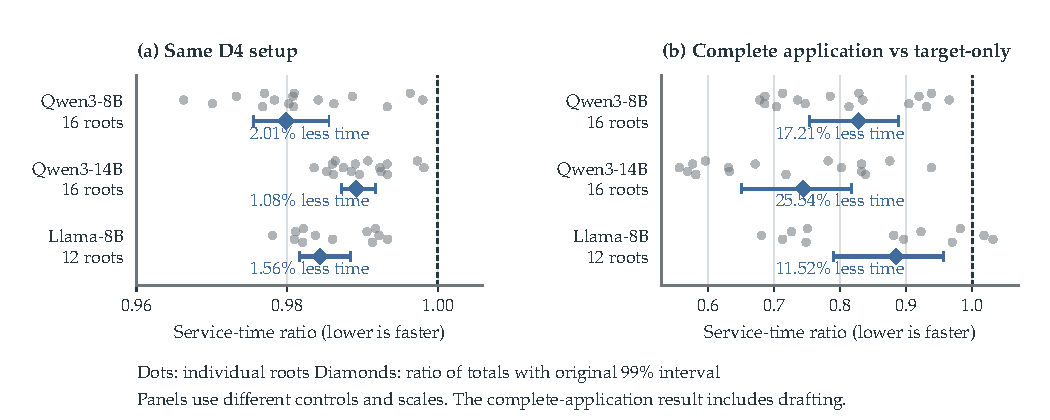
\includegraphics[width=\textwidth]{fig05_application.pdf}
\caption{The execution increment and complete speculative-application benefit. Panel (a) compares \Local-packed D4 with \Simple-loop4 D4 at the same draft setup; panel (b) compares it with the fastest measured fixed target-only M implementation. Dots sum repeated sessions within each root; diamonds are ratios of total resident time with the original 99\% paired-root intervals for five comparisons. Qwen uses 16 roots and Llama 12, each measured in four sessions. The 8B D4-arm order was fixed; the separate balanced factorial provides the stronger component attribution. The panels use separate scales.}
\label{fig:supp-application}
\end{figure}
\begin{table}[htbp]
\centering\small
\caption{Mean resident seconds per request for all six A5000 application arms. Each Qwen arm contains 64 measured requests, and each Llama arm 48. W means \Simple{} whole-graph cuts; L means \Local; L4 is backend-loop4 and P is packing. M loads target resources alone. D4 uses draft prefill microbatch four with $k=3$.}
\label{tab:supp-all-arms}
\begin{tabular}{@{}lrrrrrr@{}}\toprule
Model & W-L4-M & W-P-M & L-L4-M & L-P-M & W-L4-D4 & L-P-D4\\\midrule
\SuppApplicationRows
\bottomrule\end{tabular}
\end{table}

\begin{table}[htbp]
\centering\small
\caption{All five fixed application comparisons in each A5000 model. The numerator is L-P-D4 throughout. Each interval is a 99\% paired-root interval from that model's five-comparison family. Ratios use total resident time.}
% All five fixed application comparisons per model; generated from public timing rows.
% Requires booktabs. Numerator throughout: L_P_D4. W denotes SIMPLE.
\begin{tabular}{llrrr}
\toprule
Target & Fixed comparator & Time ratio & 99\% lower & 99\% upper \\
\midrule
Qwen3-8B & \texttt{W\_L4\_M} & 0.816506 & 0.747568 & 0.872304 \\
 & \texttt{W\_P\_M} & 0.827922 & 0.753870 & 0.888346 \\
 & \texttt{L\_L4\_M} & 0.816098 & 0.747171 & 0.872569 \\
 & \texttt{L\_P\_M} & 0.827443 & 0.753938 & 0.887542 \\
 & \texttt{W\_L4\_D4} & 0.979884 & 0.975589 & 0.985559 \\
\addlinespace
Qwen3-14B & \texttt{W\_L4\_M} & 0.740178 & 0.648295 & 0.811920 \\
 & \texttt{W\_P\_M} & 0.744608 & 0.651094 & 0.817914 \\
 & \texttt{L\_L4\_M} & 0.740286 & 0.648446 & 0.812100 \\
 & \texttt{L\_P\_M} & 0.744521 & 0.651113 & 0.817854 \\
 & \texttt{W\_L4\_D4} & 0.989193 & 0.987176 & 0.991690 \\
\addlinespace
Llama-8B & \texttt{W\_L4\_M} & 0.873640 & 0.783602 & 0.941788 \\
 & \texttt{W\_P\_M} & 0.884744 & 0.790475 & 0.956649 \\
 & \texttt{L\_L4\_M} & 0.873796 & 0.783749 & 0.941931 \\
 & \texttt{L\_P\_M} & 0.884779 & 0.790486 & 0.956653 \\
 & \texttt{W\_L4\_D4} & 0.984359 & 0.981680 & 0.988452 \\
\bottomrule
\end{tabular}

\end{table}

\begin{table}[htbp]
\centering\small
\caption{All four factorial effects and the interaction in each Qwen model. Direct effects are ratios of total service; the interaction is an equal-root geometric ratio of ratios. Intervals are 99\% paired-root percentiles in the five-comparison family.}
\begin{tabular}{@{}llrl@{}}\toprule
Model & Comparison & Ratio & Interval\\\midrule
\SuppFactorRows
\bottomrule\end{tabular}
\end{table}

\begin{table}[htbp]
\centering\small
\caption{Lifecycle costs for selected fixed controls. Resident, burst and worker clocks overlap and must not be added. A dash is an omitted field, not a zero. Workers include loading, integrity checks and primers; OS file caches were not cleared, so these are not cold-start latency claims.}
\begin{tabularx}{\textwidth}{@{}p{2.6cm}p{2.6cm}rrY@{}}\toprule
Deployment & Comparison & Resident (s) & Worker (s) & Interpretation\\\midrule
A5000 Qwen3-8B & W-P-M / L-P-D4 & 172.146 / 142.523 & 200.739 / 168.973 & Published worker totals are rounded to milliseconds.\\
A5000 Qwen3-14B & W-P-M / L-P-D4 & 294.542 / 219.318 & 662.546 / 594.559 & Measured-request bursts are 294.632 / 219.405\,s.\\
A5000 Llama-8B & L-P-M / L-P-D4 & 136.873 / 121.102 & 361.717 / 368.822 & The fastest M worker is W-P-M at 355.730\,s, a different arm from fastest resident M.\\
Windows Qwen3-8B & W-P-M / L-P-D4 & 219.810 / 155.814 & 260.240 / 192.568 & Separate deployment; input identities later reused on A5000.\\\bottomrule
\end{tabularx}
\end{table}

The Windows practical comparison gives 29.11\% less resident time and 26.00\% less worker time than the fastest fixed M. It includes the complete speculative application. Its phase account saves 96.889\,s of target work, adds 31.931\,s of draft work and 0.962\,s of other costs, for 63.996\,s net resident savings. Device-memory samples show an additional 0.705\,GiB peak for the draft-containing configuration; per-process memory peaks and energy were not measured.

The B570 resident pilot instead favors ordinary generation. Its four exposed roots and two blocks give mean times of 1.1503\,s for M and 1.8235\,s for the fastest speculative arm. A separate mechanism record has 578 local and 582 whole target graphs for 1,156 target rows, compared with 992 scalar M graphs/rows. A distinct synchronized two-root cost diagnostic saves 0.466681\,s in target work but adds 1.923330\,s in draft work and 0.210582\,s elsewhere. The different windows are not combined.

\begin{figure}[htbp]
\centering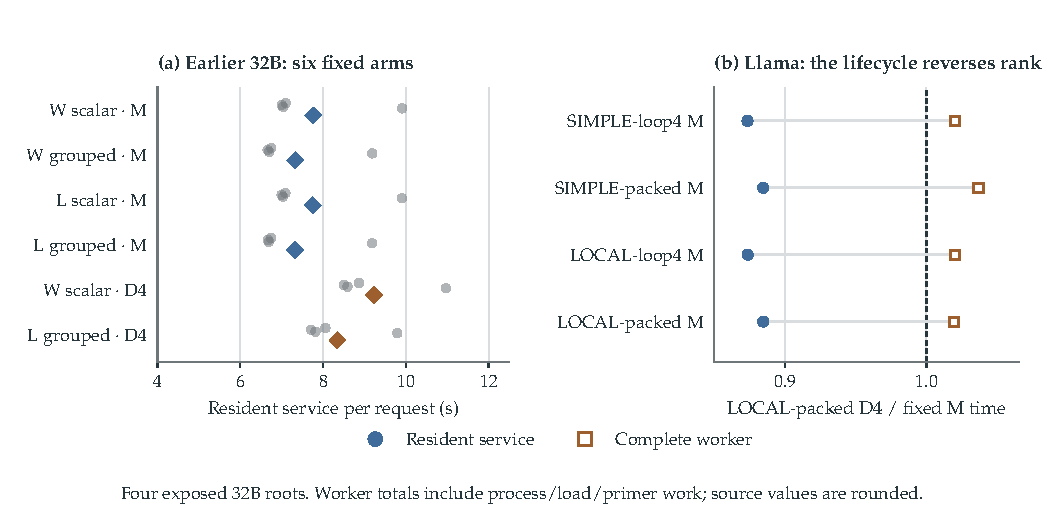
\includegraphics[width=\textwidth]{supp04_prior32b_lifecycle.pdf}
\caption{Earlier mixed-Q4 application results and the lifecycle reversal. Panel (a): the four-root 32B panel uses a graph scalar-loop control and is distinct from the later 12-root strong-backend study; all six paths are shown, including the slower speculative arms. Panel (b): Llama-8B resident and worker costs are shown for the four fixed M controls and the candidate; overlapping clocks are not stacked. Source values are public numeric projections, identified in the manifest.}
\label{fig:supp-old32}
\end{figure}

\begin{table}[htbp]
\centering\small
\caption{All six earlier Qwen3-32B mixed-Q4 arms: four exposed mathematics roots, four rounds, 16 measured requests per arm and 16 identical-root warmups. REF1L is the graph scalar-column loop and REF1G is independent grouping. The subsequent strong B control is absent from this earlier panel.}
\begin{tabular}{@{}lrr@{}}\toprule
Arm & Resident sum (s) & Mean (s)\\\midrule
\SuppPriorRows
\bottomrule\end{tabular}
\end{table}

Grouping improves this earlier panel by 5.62\% with whole cuts and 5.61\% with local cuts relative to its graph-loop control. Those effects include shared-quantization advantages that the main paper's stronger B control already obtains. Grouped D4 is 14.00\% slower than the fastest ordinary grouped arm. The strong-control operator follow-up separately uses three paired blocks in four exposed tensor cells, with one warmup and one measured operation per fresh worker. Table~\ref{tab:supp-s2} retains all cells, including mixed directions for Q6\_K/$q=4$.

\begin{table}[htbp]
\centering\small
\caption{Strong scalar-loop operator follow-up. B/G and C/B are geometric means of three paired elapsed-time ratios; ranges show observed paired minima and maxima, not confidence intervals. Equal-cell geometric ratios are 0.6390 and 0.8528. These are operator observations, distinct from the later complete service result.}
\label{tab:supp-s2}
\begin{tabular}{@{}lrrl@{}}\toprule
Cell & B/G & C/B & C/B range\\\midrule
\SuppOperatorRows
\bottomrule\end{tabular}
\end{table}
\FloatBarrier

\section{Natural-history reuse and source-derived work}
\label{sec:supp-history}
The natural two-turn pilot uses Qwen3-8B Q8 on the A5000 with capacity 4096, F16 K/V, two CPU threads and a 32-output reserve. Both arms retain backend-loop4 projections and target-only generation. The resident request timer includes reset, history rendering and tokenization, controller transport and durable per-decode accounting in the frozen host adapter. It excludes model loading, network and human waiting time, and post-response audit. These boundaries describe the experimental adapter rather than a production latency target.

The second request must reconcile its canonical history with the first request's materialized state. Table~\ref{tab:supp-history} follows the two observed transitions. The current assistant prompt ends with a four-token empty-think stub. After a capped 128-token reply, 127 body tokens are materialized and the final emitted token is pending. The next request's canonical history omits the stub, retaining the same 128 body token IDs at earlier positions. The first differing token is therefore at the start of the stub. Trimming to that common prefix is correct; reusing the old body KV would preserve the wrong positions and conditioning.

\begin{table}[htbp]
\centering\small
\caption{A timeline of the two observed history transitions. Positions are zero-based; ranges are half-open. C0 and C1 are the two free-generation conversations, not the separate supplied-history corpus. The same reconciliation is used by \Simple{} and \Local.}
\label{tab:supp-history}
\begin{tabularx}{\textwidth}{@{}p{3.7cm}p{2.2cm}p{2.2cm}Y@{}}\toprule
Transition & C0 & C1 & State consequence\\\midrule
Initial prompt, including stub & 92 tokens & 27 tokens & Four-token stub precedes the generated body.\\
After 128 emitted body tokens & KV end 219; pending 219 & KV end 154; pending 154 & The final emitted token is not yet in KV.\\
Canonical history removes stub & Body $[88,216)$ & Body $[23,151)$ & All 128 body token IDs match; their positions and prefix change.\\
Reconcile at common prefix & Keep 88; trim 131 & Keep 23; trim 131 & Remove four stub rows and 127 materialized body rows.\\
Prefill the next canonical suffix & $250-88=162$ rows & $551-23=528$ rows & Both arms recompute the required suffix before continuing.\\\bottomrule
\end{tabularx}
\end{table}

The two arms retain the same reusable earlier prefix. On later requests, older assistant turns that are already canonical can remain before the first difference. A separate CPU calculation over supplied histories predicts that 331 of 1,127 later nodes retain an earlier canonical assistant span. This is a conditional prediction for those supplied histories, not a frequency measured from free generation or a GPU saving.

The eight timed episodes sum to 36.385331\,s for whole-graph cuts and 37.920656\,s for \Local. Of the 1.535324\,s pooled difference, 1.419701\,s lies in the common sampling span. The equal-partition controls also include slower \Local{} episodes. With two conversations and two rounds, these observations do not isolate a stable local-cut penalty; they show why a saved outer call cannot by itself predict the resident result.

The proposed 89-row append provides a complementary, source-derived account. Starting at head 232, whole-call chunks are $[24,32,32,1]$ and local-call chunks $[32,32,25]$. Both retain the same ordered 23 projection tiles per fully consumed projection and 23 attention tiles per layer. Logical F32 mask storage rises from 157,696 to 182,272 bytes, while attention concatenation nodes increase from 19 to 20 per layer. The local construction additionally entails six strided-mask contiguous-copy nodes per layer, representing 24,576 logical bytes. These counts describe graph construction; actual launches, graph reuse, allocation, DRAM traffic and latency were not measured for this proposed case. \texttt{analyze\_v2.py} checks the row and tile correspondence in the fixed source analysis.
\FloatBarrier

\section{Wider execution and workload cost}
The Windows equal-work panel uses one APPS and three GSM8K origins~\cite{gsm8k}, fixed initial state, the same eight known tokens and all eight requested outputs. Its 128 measured operations and 32 primers address operation efficiency. The separate live panel uses 16 roots, prompt length at most 192, cap 96, and eight balanced order rows. Both $k=3$ and $k=7$ reserve eight outputs; 1,024 measured requests and 128 primers cover eight arms. The four primary width comparisons use 98.75\% paired-root intervals; secondary fixed-$k=7$ comparisons form a separate family.

\begin{figure}[htbp]
\centering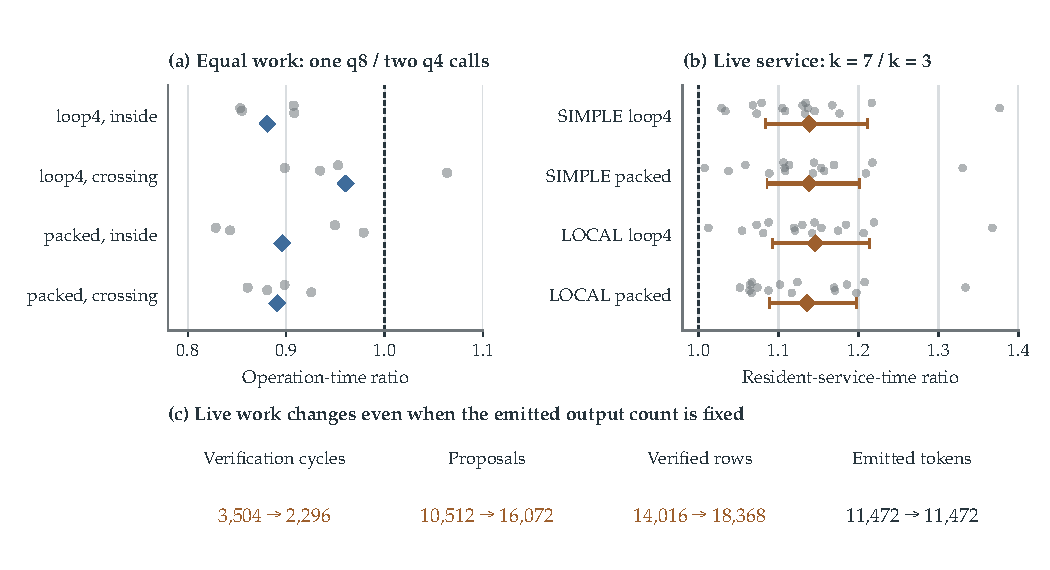
\includegraphics[width=\textwidth]{supp01_width_tradeoff.pdf}
\caption{Physical execution width and live proposal width. Equal-work $q=8$ versus two $q=4$ operations is a fixed-input comparison; $k=7$ versus $k=3$ resident generation changes the work. The live summaries use ratios of totals and 98.75\% paired-root intervals over 16 roots, with repeats clustered by root. Per-arm work counts are shared by the four methods at each $k$. These panels have different measurement boundaries.}
\end{figure}

Each live arm emits 11,472 tokens. For $k=3$/$k=7$, proposed tokens are 10,512/16,072, accepted proposals 7,928/9,152, first inspected mismatches 1,136/1,256, and unconsumed suffix tokens 1,448/5,664. Native cap/end-of-generation counts are 104/24 in each arm. Suffix waste includes post-rejection and terminal-boundary work; the aggregate counts do not separate these causes.

\begin{figure}[htbp]
\centering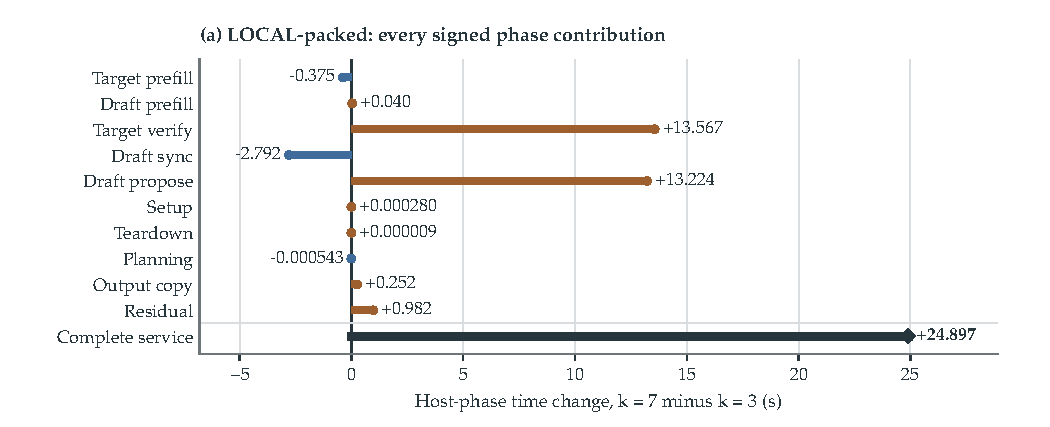
\includegraphics[width=\textwidth]{supp02_width_cost.pdf}
\caption{Where the extra live cost arises. Disjoint phase differences for \Local-packed are $k=7$ minus $k=3$ over 128 requests. Negative components save time; the net increase is 24.897\,s. Phase timers include their specified host work, synchronization and GPU execution; the residual closes the recorded service sum. These are complete-arm phase sums, not new native measurements.}
\end{figure}

The A5000 four-root pilot has 64 live measurements and 32 primers. Its \Local-packed $k=7/k=3$ ratio is 1.140572. At fixed \Local{} and $k=7$, packing/loop4 is 0.981741. A separate proposal-tape replay excludes draft work and has different target-row counts between widths, so it is not a complete-generation comparison.

\begin{table}[htbp]
\centering\small
\caption{A5000 live-width pilot. Entries are resident totals over four exposed roots and two rounds; no population interval is inferred.}
\begin{tabular}{@{}lrr@{}}\toprule
Cut / projection & $k=3$ (s) & $k=7$ (s)\\\midrule
\SuppAmpereRows
\bottomrule\end{tabular}
\end{table}

An initial A5000 equal-work comparison had unmatched first-use histories. The subsequent comparison uses 16 fresh processes, each with four warm and four measured operations, and balanced ABBA/BAAB preparation histories. It holds one exposed input, initial state and eight outputs fixed at two prefix coordinates. The complete 128-operation account gives the four process-level summaries below; mixed directions remain visible.

\begin{table}[htbp]
\centering\small
\caption{Matched-history A5000 equal-work comparison. Each cell has four fresh processes on one input; q8/q4-pair geometric means and observed process ranges are descriptive.}
\begin{tabular}{@{}lrrl@{}}\toprule
Projection & Prefix & Geometric ratio & Process range\\\midrule
\SuppMatchedRows
\bottomrule\end{tabular}
\end{table}
\FloatBarrier

\section{Boundary counterexamples and numerical migration}
The final B570 append panel has 12 fixed cells, three paths and three paired repeats, with 108 measured operations and 108 corresponding warmups. At $q=32$ it retains the registered last-only output request. Its timer begins after valid state preparation and includes phase binding, native decode, synchronization and copying the requested vector. Caller batch preparation and state import are outside it. Earlier geometries remain relevant because a $16+16$ crossing can preserve different surrounding work from a $1+31$ crossing.

\begin{figure}[htbp]
\centering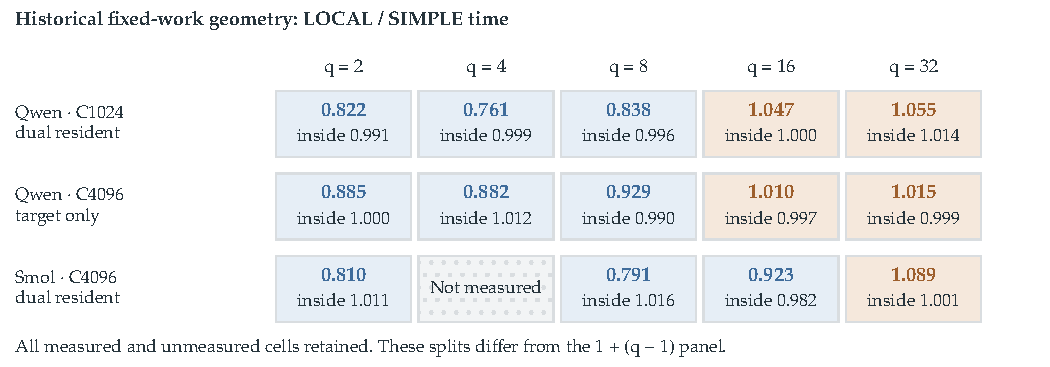
\includegraphics[width=\textwidth]{supp03_historical_geometry.pdf}
\caption{Earlier local-cut geometries, including reversals. Crossing cells are paired with inside controls; a missing cell is shown as unmeasured, not zero. These historical fixed-cell timings use their original measurement boundaries. They establish sensitivity to split geometry, not a population estimate or an isolated capacity effect.}
\end{figure}

The modern RTX comparison extracts a $4096\times4096$ Q8 projection with $q=8$ from one captured activation. U uses the upstream quantizer and few-row projection~\cite{llama_cpp_fewrow}; B retains the old reference. Table~\ref{tab:supp-rtx-variants} distinguishes the implementations. Ordinary launches with CUDA graphs disabled and the recorded programmatic-launch setting are timed using GPU events. Allocation, copies and checks are excluded; host-submission gaps can remain within an event window. The full quantization-plus-projection and projection-only boundaries have 12 paired repeats each, totaling 48 samples. Ratios are reconstructed from event duration divided by batch repetitions, avoiding rounding in the printed per-operation column.

\begin{table}[htbp]
\centering\small
\caption{Extracted RTX variants on the captured input. Register and shared-memory figures describe the projection kernel. Shared memory is per thread block; registers are per thread. No spilling is reported. C, C1 and U are measured in separate sessions against their respective B, so C/C1 is not a paired intervention. Compiler resources do not measure achieved occupancy or memory traffic.}
\label{tab:supp-rtx-variants}
\begin{tabularx}{\textwidth}{@{}p{0.65cm}Y>{\raggedright\arraybackslash}p{3.25cm}>{\raggedright\arraybackslash}p{2.5cm}r@{}}\toprule
Path & Execution change & Numerical contract & Projection resources & Complete / B\\\midrule
B & Two four-column groups in separate block groups; old packed path & Old quantizer and DP4A projection path & 63 registers; 3\,KiB static shared & 1\\
C & Two arithmetic groups in one block, reusing register-held weight fragments & Old contract, qualified on the captured case & 91 registers; 6\,KiB static shared & 1.1264\\
C1 & Sequential groups in one block, with an added barrier and no cross-group register-weight reuse & Old contract, qualified on the captured case & 64 registers; 3\,KiB static shared & 1.0261\\
U & Upstream few-row integer MMA and asynchronous weight staging & Modern quantizer and arithmetic; differs from B & 244 registers; 68\,KiB dynamic shared & 0.6129\\\bottomrule
\end{tabularx}
\end{table}

\begin{figure}[htbp]
\centering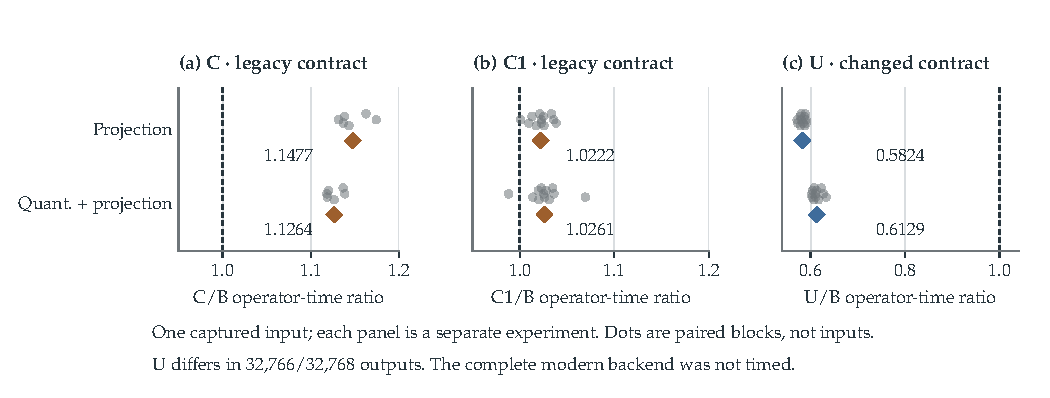
\includegraphics[width=\textwidth]{supp05_rtx_contracts.pdf}
\caption{Extracted RTX operator alternatives under distinct numerical contracts. Legacy-compatible C and C1, and modern upstream U, come from separate sessions and are not directly paired with one another. Points retain all paired repeat ratios for each boundary. U/B complete-operator time is 0.612924 with a 95\% paired-repeat interval [0.607906, 0.618665]; projection-only time is 0.582391. U does not preserve B's quantization or output bytes. The earlier old-oracle qualification failure and the unrun complete default backend have no timing point.}
\end{figure}

An earlier attempt to qualify the upstream path against a strict CPU-round-to-nearest oracle fails before timing. The subsequent study explicitly binds U's own contract and compares a valid modern numerical alternative. Static API checks for a complete current default backend pass without loading a model; full-backend numerical qualification and service timing remain unrun.
\FloatBarrier
